\documentclass[12pt]{article}

\usepackage[a4paper,margin=1in]{geometry}
\usepackage[T1]{fontenc}
\usepackage[utf8]{inputenc}
\usepackage{lmodern}
\usepackage{setspace}
\usepackage{graphicx}
\usepackage{booktabs}
\usepackage{array}
\usepackage{tabularx}
\usepackage{longtable}
\usepackage{amsmath}
\usepackage{xcolor}
\usepackage{hyperref}
\usepackage{caption}
\usepackage{float}
\usepackage{adjustbox}
\usepackage{tikz}
\usetikzlibrary{arrows.meta,positioning,calc,shapes.geometric,fit,backgrounds}

\hypersetup{
  colorlinks=true,
  linkcolor=blue!60!black,
  citecolor=blue!60!black,
  urlcolor=blue!60!black,
  pdftitle={Agentic Multimodal Foley System Report},
  pdfauthor={GenAI Music In Video Team}
}

\setstretch{1.2}
\setlength{\parskip}{0.55em}
\setlength{\parindent}{0pt}
\setlength{\emergencystretch}{2em}
\newcolumntype{P}[1]{>{\raggedright\arraybackslash}p{#1}}

\title{}
\author{}
\date{}

\begin{document}

\begin{titlepage}
\centering
\vspace*{2.8cm}
{\Large \textbf{Template 1 Technical Report}}\\[1.0cm]
{\LARGE \textbf{Agentic Multimodal System for Video-Grounded Foley Generation}}\\[1.2cm]
{\large GenAI Music In Video Project}\\[0.6cm]
{\large April 2026}\\[2.0cm]
{\large \textbf{Abstract}}\\[0.4cm]
\begin{minipage}{0.88\textwidth}
\centering
This report documents an agentic multimodal pipeline that transforms silent video into synchronized Foley audio through staged perception, planning, synthesis, verification, and iterative control. The system operationalizes agentic behavior by separating strategic decisions from model inference, introducing explicit uncertainty controls, and exposing internal reasoning events through a live interface. The report presents architecture rationale, model-selection arguments, end-to-end control flow, failure handling logic, and evaluation methodology, with an emphasis on verifier disagreement analysis, cross-modal agreement checks, and self-consistency diagnostics.
\end{minipage}
\vfill
{\large Department Submission Draft}
\end{titlepage}

\pagenumbering{roman}
\setcounter{page}{1}
\tableofcontents
\newpage
\pagenumbering{arabic}
\setcounter{page}{1}

\section{Introduction and Problem Framing}

The project targets a difficult multimodal generation problem: producing believable and temporally aligned Foley audio from visual input while maintaining transparent and controllable reasoning. A single model call is insufficient because the problem combines at least four distinct cognitive demands that conflict when collapsed into one pass. The system must first identify temporally meaningful visual moments, then convert those moments into acoustically specific descriptions, then synthesize audio clips, and finally judge quality and grounding before deciding whether additional attempts are justified. Each stage depends on intermediate artifacts that require validation rather than blind chaining.

The implemented system therefore adopts an explicit agentic architecture with bounded roles. Perception extracts and summarizes sound-relevant visual evidence from sampled frames. Planning converts the evidence into timestamped audio directives. Execution synthesizes candidate waveforms from prompts. Verification scores semantic audio-text alignment with an ensemble CLAP strategy, after which a controller decides whether to accept, retry with rewrite, retry with the best prior prompt, or terminate with the best available candidate. This staged process is exposed through a runtime event stream so that both developers and evaluators can inspect how decisions were made under uncertainty.

\section{Task Decomposition as an Agentic Contract}

The decomposition is deliberately strict because temporal alignment and semantic grounding must be handled separately. The first contract is between visual perception and planning. Perception must output a timeline-style textual artifact that encodes events and acoustic cues rather than visual descriptions alone. The second contract is between planning and execution. Planning must emit JSON-structured event objects with bounded timestamps and durations so synthesis can proceed deterministically. The third contract is between execution and verification. Execution returns concrete audio samples, and verification maps each sample back to the originating prompt through CLAP-based similarity scoring. The fourth contract is between verification and the controller, where uncertainty is represented not only by raw score magnitude but also by verifier disagreement and cross-modal mismatch.

This design makes failure locality explicit. If planning returns malformed or empty events, fallback planning can inject a conservative ambient event without collapsing the full run. If verification identifies disagreement across scoring models, acceptance can be blocked even when one score appears strong. If cross-modal lexical grounding is weak, the controller can force rewrite behavior. Agentic behavior emerges from these explicit handoff rules rather than from an unconstrained monolithic prompt.

\section{System Architecture}

The runtime consists of three connected surfaces: the orchestration core, the model-serving API, and the WebSocket application layer that streams reasoning to the user interface. The orchestration core in \texttt{main.py} owns stage coordination, thresholding, retries, trace construction, and artifact stitching. The model-serving API in \path{server/multi_model_api.py} hosts stage-specific model endpoints with resource-aware loading and optional offloading. The WebSocket bridge in \path{server/agent_ws_api.py} receives run requests, executes the orchestrator asynchronously, and streams semantically typed events to the frontend.

\begin{figure}[H]
\centering
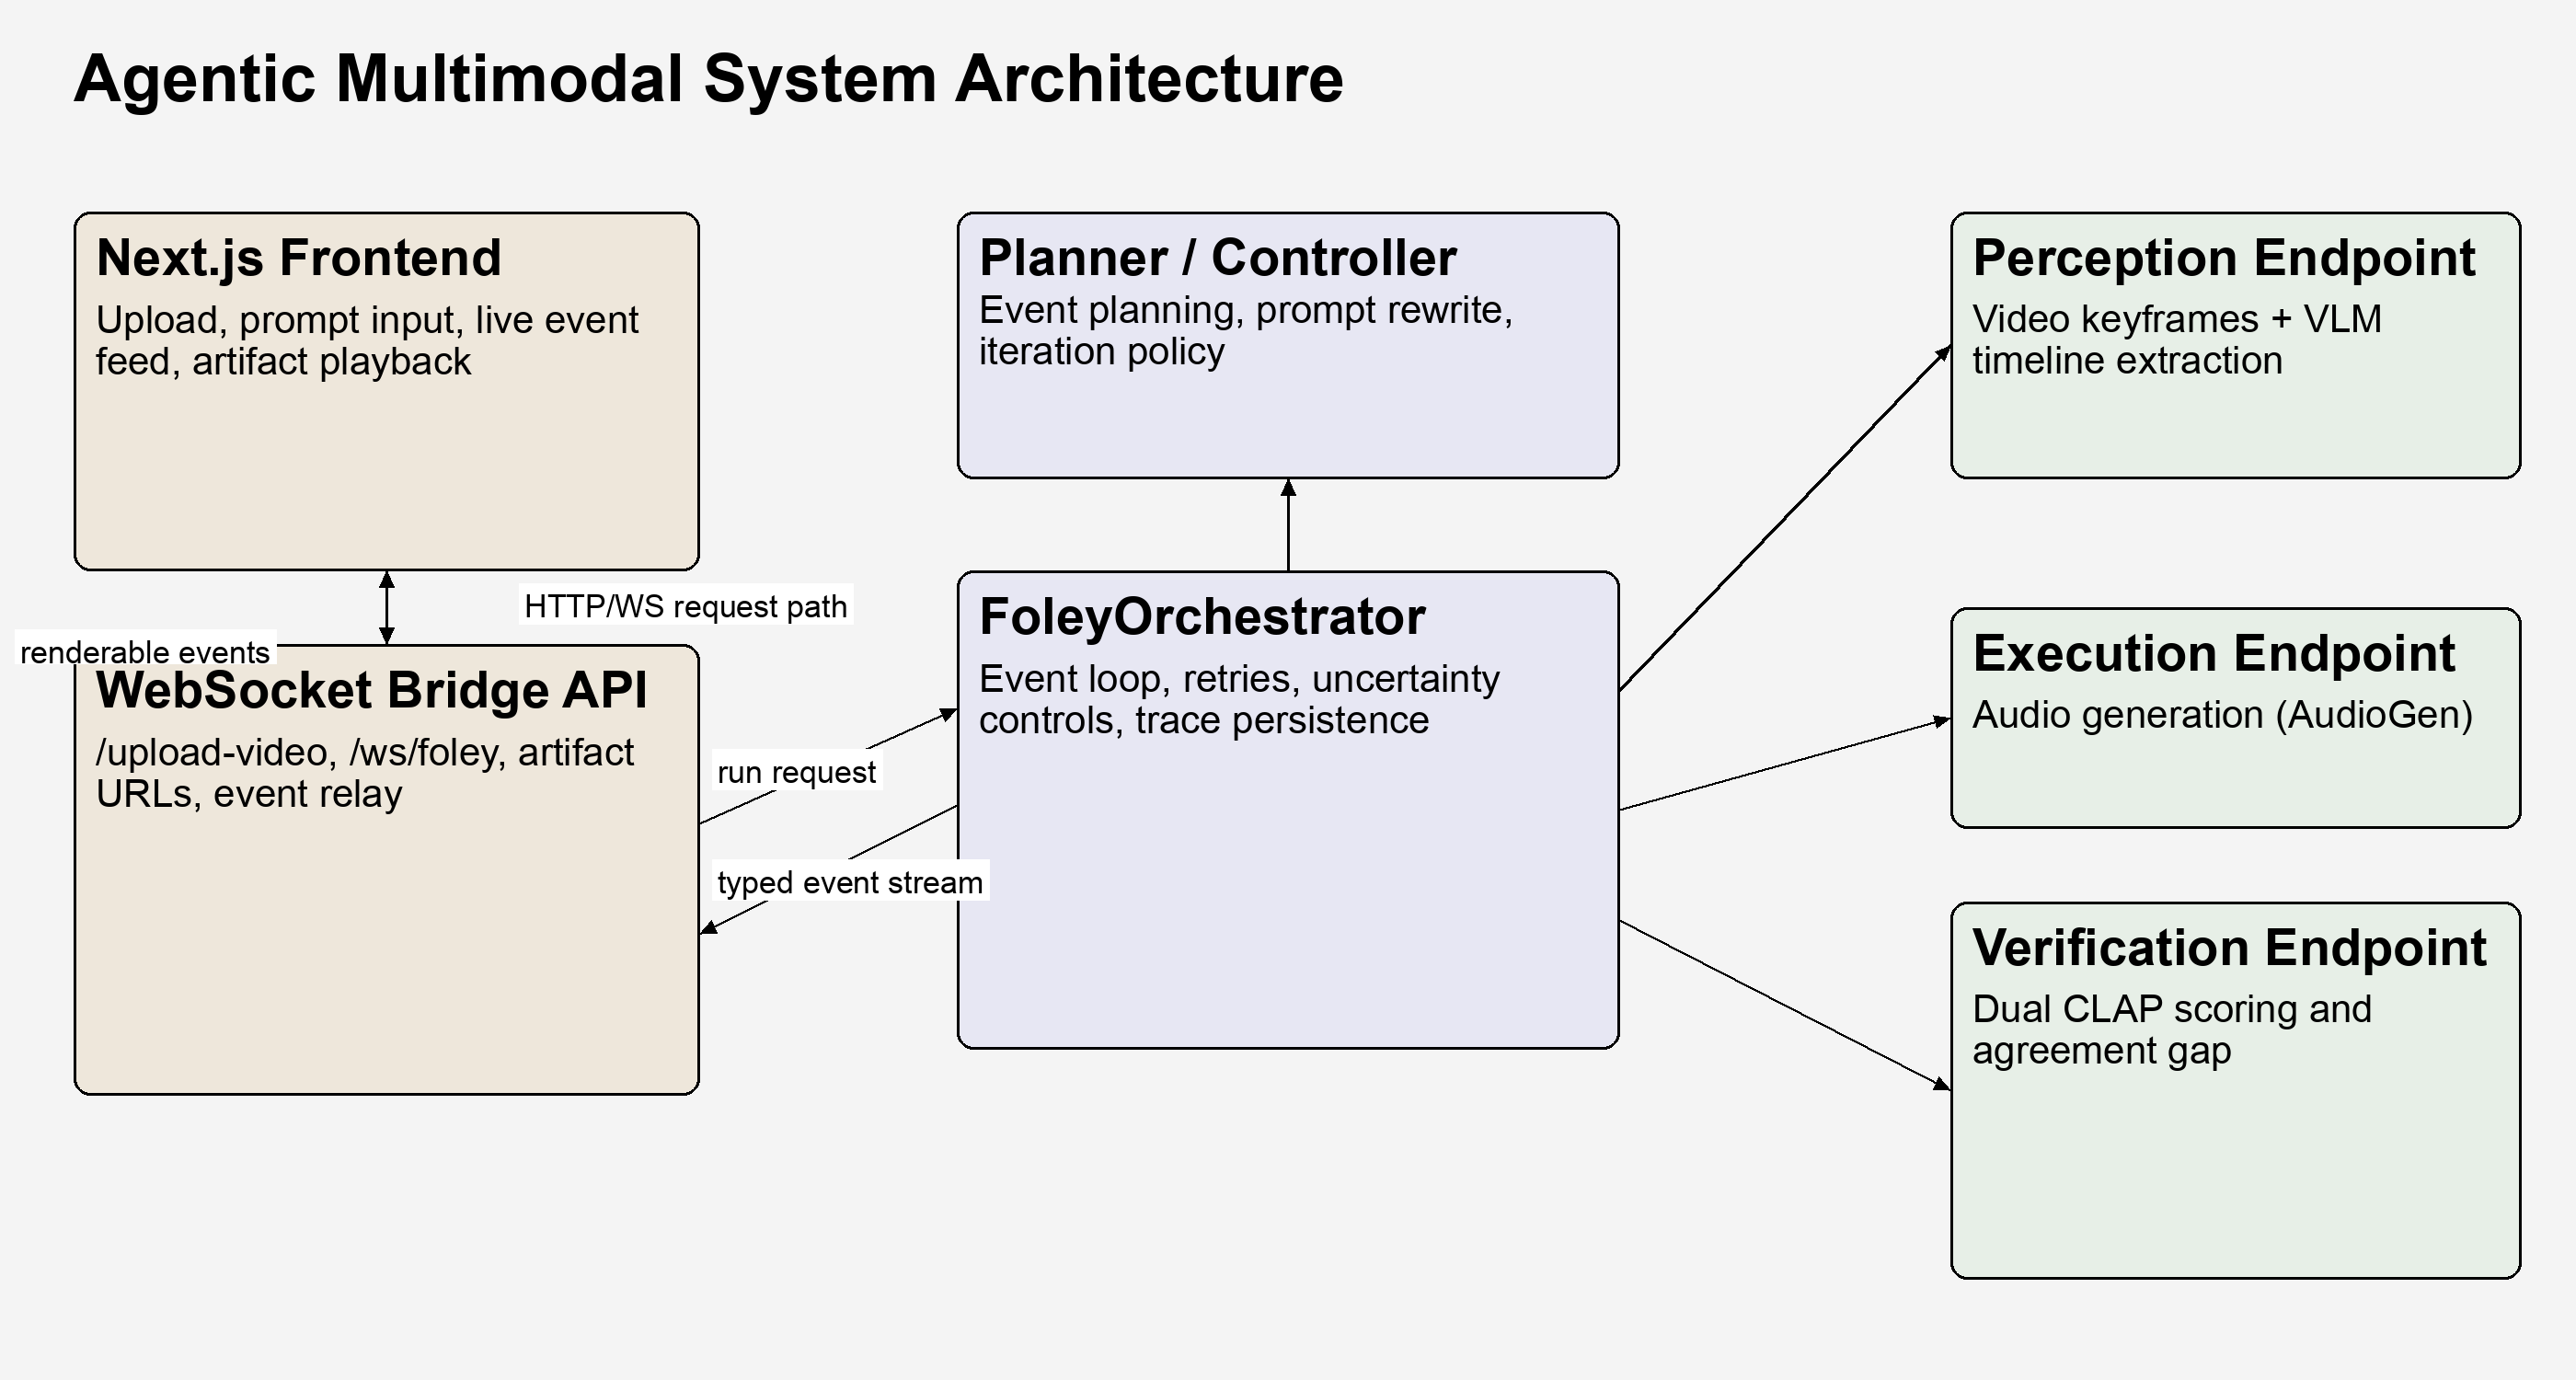
\includegraphics[width=\textwidth]{assets/architecture_diagram.png}
\caption{Top-level architecture of the agentic multimodal Foley system rendered as a static image to prevent node/label overlap.}
\label{fig:system-architecture}
\end{figure}

\section{Model Selection Rationale}

Model selection balances semantic competence, modality fit, deployment practicality, and control observability. The perception stage requires a vision-language model capable of integrating multiple frame inputs and producing coherent timeline text. This workload prioritizes cross-frame reasoning and descriptive robustness over generation diversity, so an instruction-tuned VLM is appropriate. The planner and controller stage requires high instruction adherence and JSON compliance under strict schemas; this stage benefits from chat-completion models with stable formatting behavior because malformed plan output creates cascading failures.

Execution uses a text-to-audio model optimized for short conditioned generation with acceptable latency. This stage is intrinsically stochastic, so the orchestration design assumes imperfect first-pass results and wraps synthesis in a retry-and-verification loop. Verification uses CLAP embeddings because the core quality question is semantic agreement between textual intent and produced audio. A dual-verifier strategy is used to reduce overconfidence from any one encoder. The final score is conservatively taken as the minimum of the two verifier scores, while score gap acts as an independent uncertainty measure. This conservative fusion is intentionally risk-averse: it lowers nominal scores, but it materially improves trustworthiness of acceptance decisions.

The runtime API supports stage-specific model configuration through environment variables and command-line arguments, enabling reproducible ablations and hardware-aware deployment. Optional model offloading after each request controls VRAM pressure and improves compatibility with constrained machines at the cost of latency. This tradeoff is operationally meaningful for coursework demonstrations where deterministic completion is often more important than absolute throughput.

\setlength{\tabcolsep}{3pt}
\renewcommand{\arraystretch}{1.15}
\footnotesize
\begin{longtable}{|P{1.8cm}|P{2.9cm}|P{1.6cm}|P{4.2cm}|P{4.2cm}|}
\caption{Selected models with stage roles, scale, operational dimensions, and rationale.}
\label{tab:model-selection}\\
\hline
\textbf{Stage} & \textbf{Chosen Model(s)} & \textbf{Scale} & \textbf{Operational Dimensions in This System} & \textbf{Selection Rationale} \\
\hline
\endfirsthead
\hline
\textbf{Stage} & \textbf{Chosen Model(s)} & \textbf{Scale} & \textbf{Operational Dimensions in This System} & \textbf{Selection Rationale} \\
\hline
\endhead
\hline
\endfoot
Perception & Qwen / Qwen2-VL-2B-Instruct & \(\sim\)2B & Up to 12 sampled keyframes by default, each preprocessed to 896\(\times\)896 RGB before VLM inference; output is timeline text for planning. & Good multimodal instruction following at moderate runtime cost, suitable for extracting sound-relevant cues from sparse frames. \\
\hline
Planner & Qwen / Qwen2.5-7B-Instruct (API default) & \(\sim\)7B & Input is VLM timeline text; output is strict JSON events with \texttt{timestamp\_sec}, \texttt{duration\_sec}, and \texttt{original\_prompt}. & Stronger schema compliance and temporal decomposition stability than smaller planning models. \\
\hline
Controller / Rewriter & llama-3.3-70b-versatile (orchestrator setting) & 70B & Input is event state, score history, and thresholds; output is one action among \texttt{ACCEPT}, \texttt{RETRY\_REWRITE}, \texttt{RETRY\_BEST}, \texttt{STOP\_BEST} plus rationale and confidence. & Larger reasoning capacity improves iterative decision quality and prompt-refinement reliability under uncertainty. \\
\hline
Execution & facebook / audiogen-medium & Medium & Input is text prompt plus duration (seconds); output is generated waveform exported as mono WAV at 16 kHz. & Practical quality-latency balance for short Foley clips with controllable generation duration. \\
\hline
Verification (primary) & laion / clap-htsat-fused & CLAP encoder & Input is prompt text and audio resampled to 48 kHz; output is a scalar similarity logit. & Provides a robust text-audio alignment signal for acceptance control. \\
\hline
Verification (secondary) & laion / larger\_clap\_general & Larger CLAP encoder & Same interface as primary verifier; adds disagreement gap \(\Delta = |s_1 - s_2|\) and agreement flag using threshold \(\delta\). & Model diversity reduces single-verifier bias and supports uncertainty-aware gating. \\
\hline
\end{longtable}
\normalsize

\section{Agentic Loop and Inter-Model Interactions}

The loop begins with either a direct prompt-only mode or a video-grounded mode. In video-grounded mode, keyframe extraction uses frame-difference thresholding and optional downsampling to cap visual token load while preserving temporal diversity. The perception prompt enforces timeline formatting so that downstream planning receives acoustically useful and temporally bounded evidence. Planning converts that evidence into event objects with \texttt{timestamp\_sec}, \texttt{duration\_sec}, and \texttt{original\_prompt}. If planning fails, a conservative ambient fallback is injected to preserve forward progress.

For each planned event, execution synthesizes candidate audio using the current prompt. Verification computes dual CLAP scores and returns primary score, secondary score, gap, and agreement status. The orchestration layer normalizes the final score into a decision scale and runs cross-modal agreement checks between expected scene keywords and prompt tokens. The controller then chooses an action among acceptance and retry modes. The loop continues until acceptance, explicit stop-best termination, or retry budget exhaustion.

\begin{figure}[H]
\centering
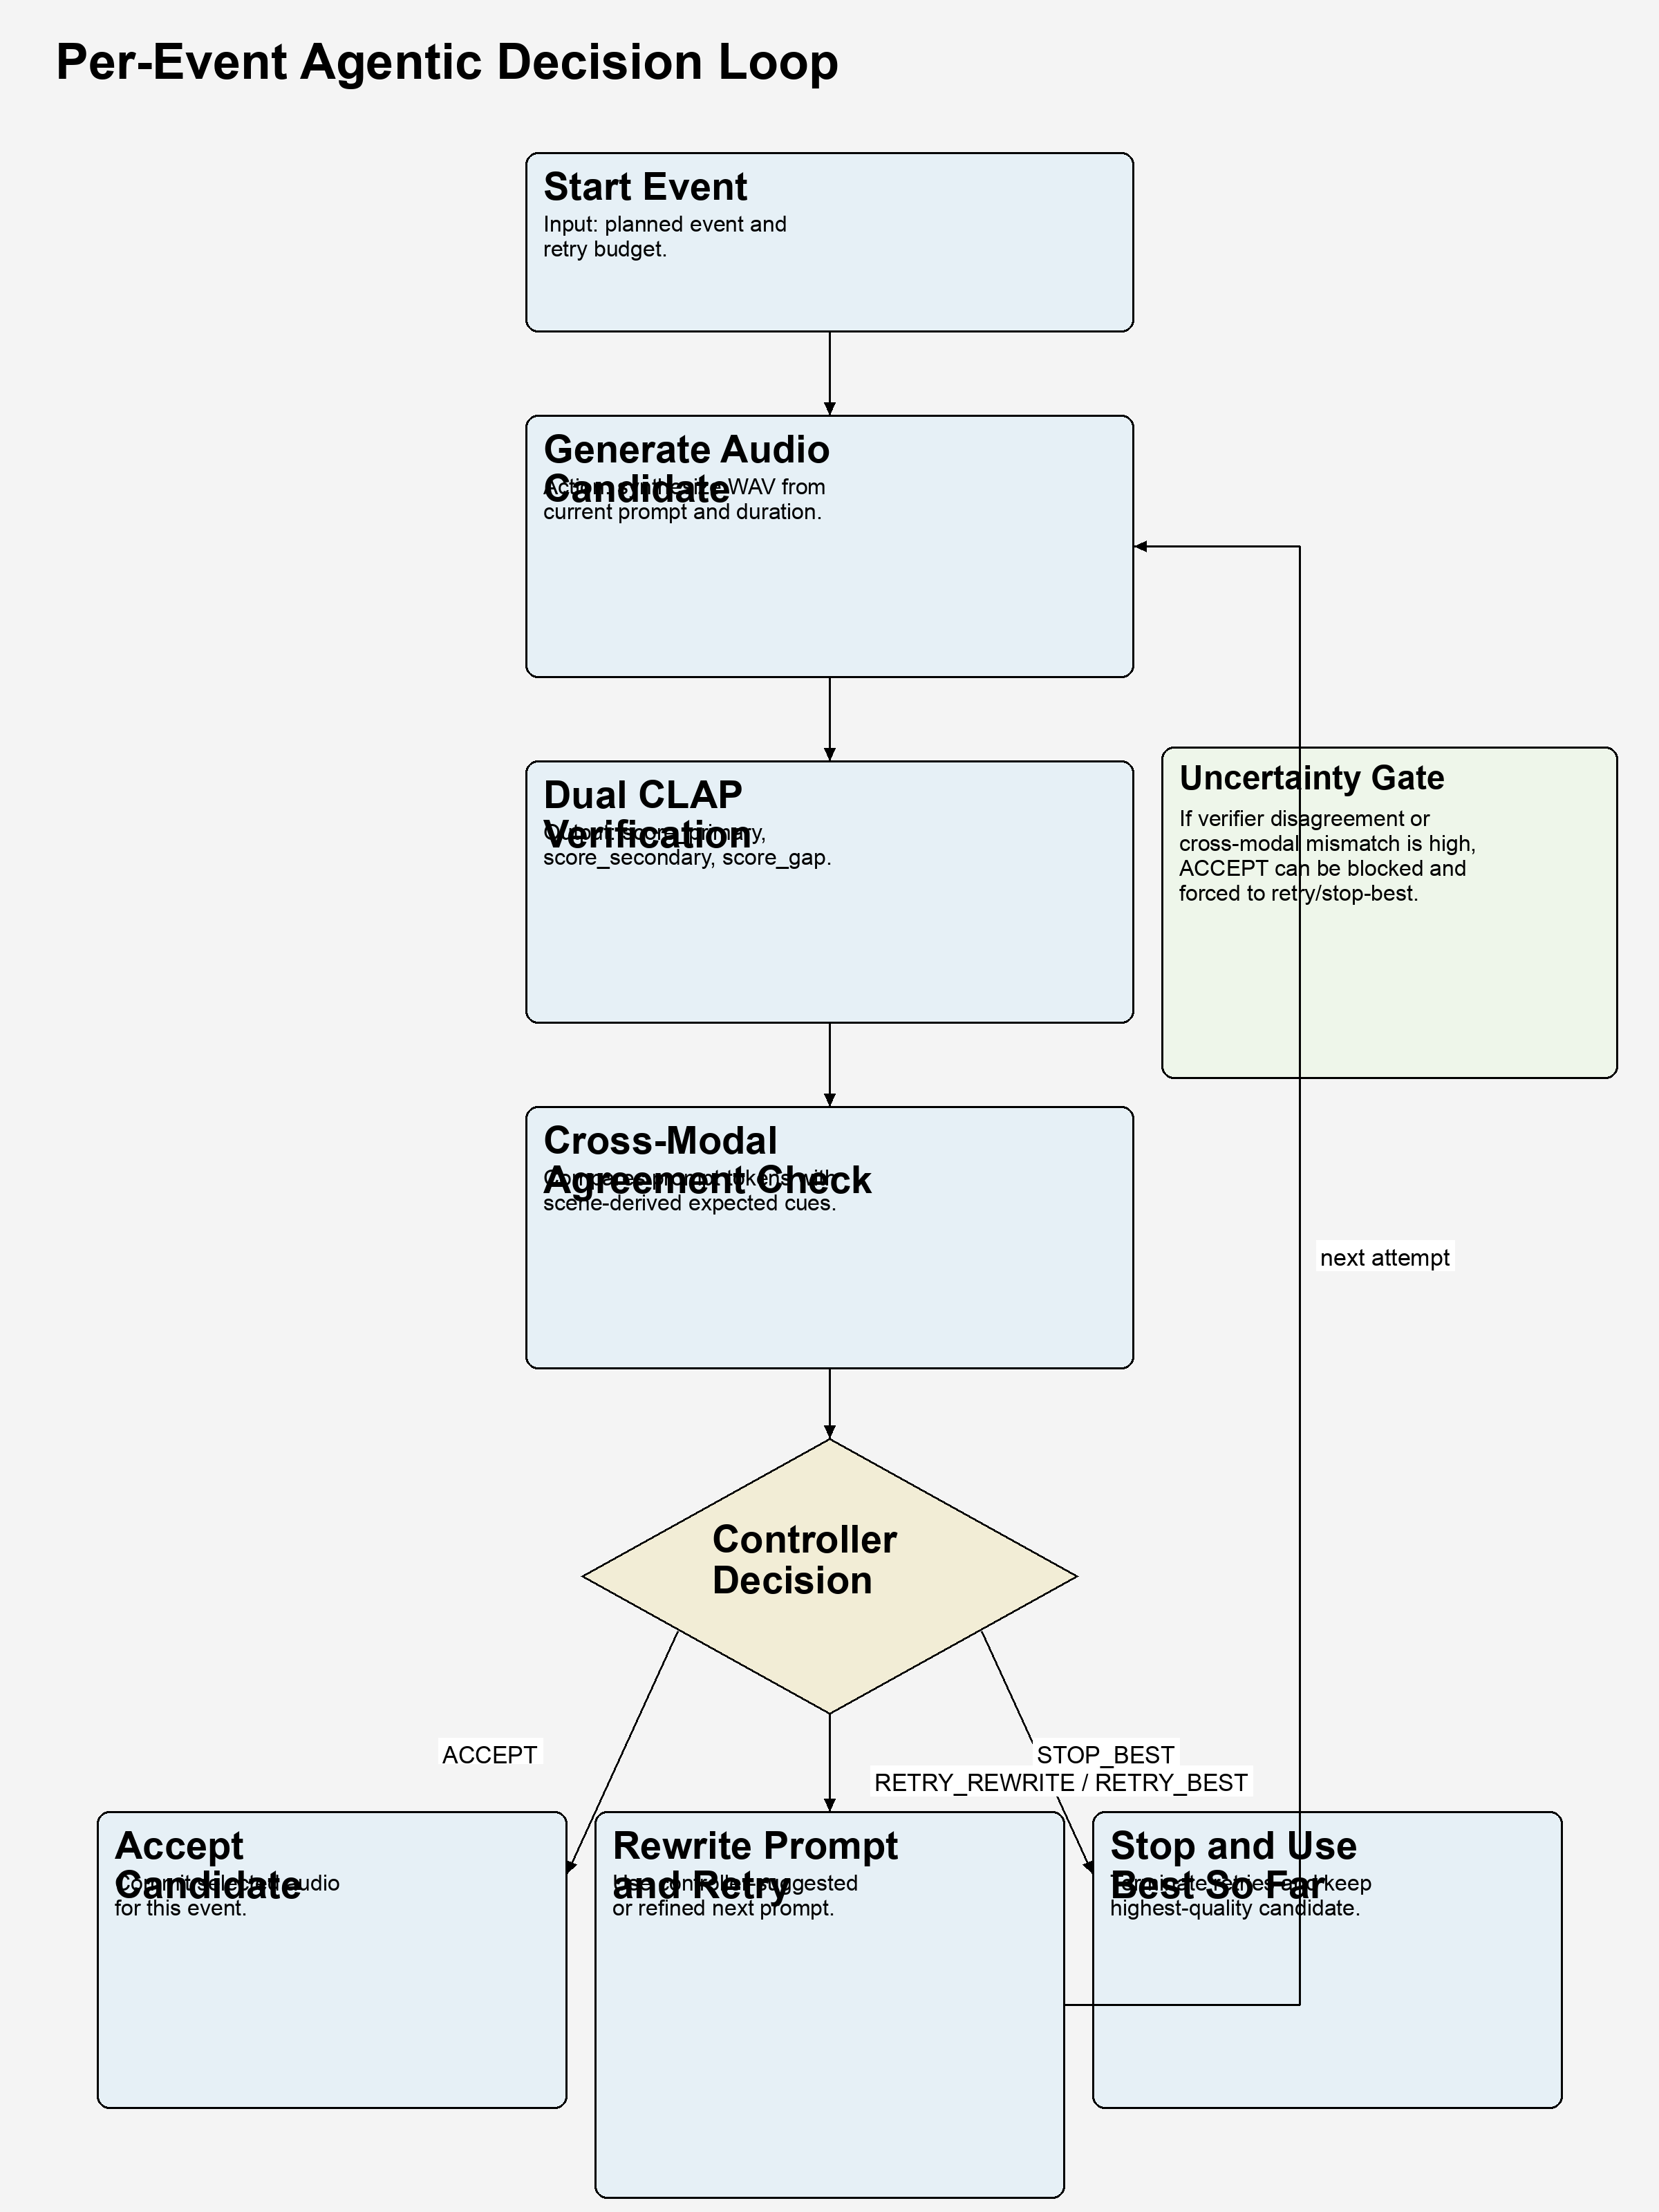
\includegraphics[width=0.78\textwidth]{assets/agent_loop_diagram.png}
\caption{Per-event agentic loop rendered as a static image to maintain clean edge labels and retry-loop routing.}
\label{fig:agent-loop}
\end{figure}

\section{Retry Policy, Fallback Strategy, and Uncertainty Gating}

The retry policy is not a simple threshold comparator. Acceptance can be blocked when uncertainty indicators are active, even if nominal quality appears sufficient. The first uncertainty indicator is verifier disagreement, measured as the CLAP score gap between primary and secondary models. The second is cross-modal mismatch, measured by overlap between expected scene keywords and the active prompt. If either indicator fails, uncertainty is recorded in the attempt trace. If the controller proposes \texttt{ACCEPT} during uncertainty, acceptance is overridden to retry behavior or forced \texttt{STOP\_BEST} on the final attempt.

This gating behavior prevents brittle acceptance of semantically dubious outputs. It also creates auditable reasoning artifacts. Each attempt stores score values, uncertainty reasons, controller rationale, confidence estimate, and action source. When runs finish, the system persists a report JSON that includes event-wise traces and selected prompts. This persistent trace design materially improves reproducibility of failure analysis and supports structured postmortem review in coursework settings where evidence quality is graded.

\begin{figure}[H]
\centering
\begin{adjustbox}{max width=\textwidth}
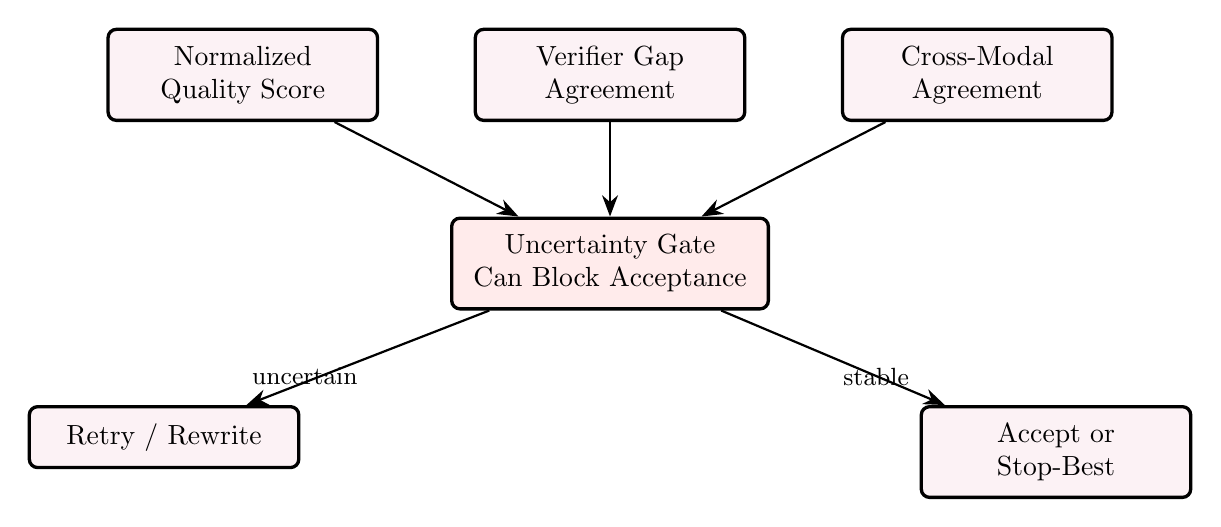
\begin{tikzpicture}[
  node distance=1.05cm and 1.2cm,
  state/.style={draw, rounded corners=3pt, very thick, fill=purple!5, align=center, text width=3.0cm, inner sep=6pt},
  gate/.style={draw, rounded corners=3pt, very thick, fill=red!8, align=center, text width=3.6cm, inner sep=6pt},
  arrow/.style={-{Stealth[length=2.7mm]}, thick}
]

\node[state] (score) {Normalized\\ Quality Score};
\node[state, right=of score] (agree) {Verifier Gap\\ Agreement};
\node[state, right=of agree] (xmod) {Cross-Modal\\ Agreement};
\node[gate, below=1.2cm of agree] (block) {Uncertainty Gate\\ Can Block Acceptance};
\node[state, below left=1.2cm and 1.9cm of block] (retry) {Retry / Rewrite};
\node[state, below right=1.2cm and 1.9cm of block] (accept) {Accept or\\ Stop-Best};

\draw[arrow] (score) -- (block);
\draw[arrow] (agree) -- (block);
\draw[arrow] (xmod) -- (block);
\draw[arrow] (block) -- node[below left, font=\small]{uncertain} (retry);
\draw[arrow] (block) -- node[below right, font=\small]{stable} (accept);

\end{tikzpicture}
\end{adjustbox}
\caption{Acceptance is conditioned on both quality and uncertainty agreement checks, not quality alone.}
\label{fig:uncertainty-gate}
\end{figure}

\section{CLAP-Based Verification Details}

CLAP verification maps text and audio into a shared embedding space, enabling direct semantic similarity scoring. The system computes scores from two CLAP models and introduces conservative score fusion to reduce false confidence. Let $s_1$ and $s_2$ denote primary and secondary similarity scores for a prompt-audio pair. The deployed conservative score is $s_{\text{final}} = \min(s_1, s_2)$, while disagreement is measured as $\Delta = |s_1 - s_2|$. Agreement is declared when $\Delta \leq \delta$, where $\delta$ is the configured verifier gap tolerance.

To stabilize controller behavior across model ranges, the orchestration layer maps raw scores to a normalized decision scale. If $s_{\min}$ and $s_{\max}$ are configured calibration bounds, then normalized quality is computed as
\[
q = \mathrm{clip}_{[0,1]}\left(\frac{s_{\text{final}} - s_{\min}}{s_{\max} - s_{\min}}\right).
\]
This normalized value drives retry policy and acceptance comparisons while preserving raw values for trace transparency. The normalized form also improves comparability across runs that may use different verifier model pairs.

\section{Cross-Modal Agreement and Self-Consistency Diagnostics}

Cross-modal agreement complements CLAP by checking whether prompts preserve cues extracted from visual context. Expected keywords are derived from the perception timeline and compared against the current synthesis prompt after token normalization and stopword filtering. The resulting overlap ratio acts as a lightweight semantic grounding signal. Although this lexical method is approximate, it is computationally cheap and catches practical errors such as prompt drift toward irrelevant sounds.

Self-consistency is applied to planning by sampling multiple plan generations from identical visual logs and measuring structural stability. The diagnostics include event-count variance, average timestamp deviation, and prompt-token Jaccard overlap. A stable plan is selected by median-count proximity and alignment statistics. This mechanism identifies fragile plan generation behavior before costly synthesis and provides a principled fallback point when planner outputs are unstable.

\section{Demonstration Interface and Observability}

The frontend is designed as an inspection surface rather than a black-box trigger button. Users can upload video, initiate runs, and watch typed reasoning events in chronological order. The event taxonomy includes perception events, planning completion, self-consistency metrics, verifier ensemble results, cross-modal checks, uncertainty flags, and controller decisions. Final artifacts are returned as playable media links from the backend artifact server. This structure turns a model demo into an auditable system demo, which is a central requirement for credible agentic evaluation.

The WebSocket bridge decouples long-running model inference from UI responsiveness through queued event callbacks. This avoids blocking behavior and allows progressive rendering of intermediate decisions. By streaming event payloads with explicit type labels, the interface can map system internals directly to user-visible explanations. Observability is therefore not an afterthought; it is an architectural component that supports both debugging and academic reporting.

\section{Evaluation Protocol and Baselines}

The project is structured to support three evaluation conditions. The first condition is the full agentic system with retries, uncertainty gating, cross-modal agreement checks, and dual-verifier scoring. The second condition is a single-pass baseline that performs perception, planning, synthesis, and one verification call without iterative control decisions. The third condition is a hand-designed non-agentic workflow where prompts are manually authored from video inspection and then synthesized and scored once. Comparison across these conditions should report success rate under a task-specific acceptance criterion, average final score, retry cost, and disagreement incidence.

Failure analysis should be carried out per event rather than only per video because localized failures are common in temporally dense scenes. The trace JSON produced by the orchestrator enables disagreement analysis by exposing per-attempt controller actions, uncertainty reasons, and score trajectories. A rigorous report should include cases where high nominal similarity was blocked by uncertainty checks, cases where rewrites improved cross-modal agreement, and cases where stop-best prevented excessive compute without material quality gain.

\section{Limitations and Reflection on Agentic Benefit}

Agentic behavior is most beneficial when quality cannot be determined from one signal and when actions are expensive enough to justify staged control. This Foley task satisfies both conditions because synthesis is stochastic and multimodal alignment is ambiguous. The controller materially improves reliability by separating decision policy from generation. Cross-model verification and cross-modal agreement checks provide complementary uncertainty views that reduce overconfident acceptance.

The design still has limitations. Keyword-based cross-modal checks are coarse and may miss nuanced acoustic relevance. CLAP similarity, while useful, is not a full perceptual quality metric and can be biased by prompt phrasing. Planning self-consistency measures structure but not human plausibility. The current fallback strategies prioritize robustness over creativity, which can compress expressive range. Future improvements can include stronger scene-audio grounding models, richer verifier ensembles, and a calibration study linking automatic scores to human pairwise judgments.

\section{Conclusion}

The implemented system demonstrates that practical agentic multimodal generation can be achieved through explicit decomposition, typed stage contracts, conservative verification, and policy-level retry control. The architecture is intentionally transparent, exposing internal state transitions and uncertainty signals through a live interface and persistent traces. This combination of operational reliability and observability aligns with Template 1 expectations and provides a reproducible foundation for rigorous baseline comparison and deeper empirical study.

\section{References}

\begin{thebibliography}{99}

\bibitem{radford2021clip}
Alec Radford, Jong Wook Kim, Chris Hallacy, Aditya Ramesh, Gabriel Goh, Sandhini Agarwal, Girish Sastry, Amanda Askell, Pamela Mishkin, Jack Clark, Gretchen Krueger, and Ilya Sutskever.
Learning Transferable Visual Models From Natural Language Supervision.
\textit{Proceedings of the 38th International Conference on Machine Learning}, 2021.

\bibitem{wu2023audioclip}
Ho-Hsiang Wu, Prem Seetharaman, Kundan Kumar, and Juan Pablo Bello.
WavCaps: A ChatGPT-Assisted Weakly-Labelled Audio Captioning Dataset for Audio-Language Multimodal Research.
\textit{arXiv preprint arXiv:2303.17395}, 2023.

\bibitem{elizalde2023clap}
Benjamin Elizalde, Soham Deshmukh, Huaming Wang, and Bhiksha Raj.
CLAP Learning Audio Concepts From Natural Language Supervision.
\textit{ICASSP 2023}, 2023.

\bibitem{copet2024simple}
Jade Copet, Felix Kreuk, Itai Gat, Yossi Adi, and Alexandre Défossez.
Simple and Controllable Music Generation.
\textit{Advances in Neural Information Processing Systems}, 2024.

\bibitem{openai2023gpt4v}
OpenAI.
GPT-4V(ision) System Card.
\textit{OpenAI Technical Report}, 2023.

\bibitem{yao2023react}
Shunyu Yao, Jeffrey Zhao, Dian Yu, Nan Du, Izhak Shafran, Karthik Narasimhan, and Yuan Cao.
ReAct: Synergizing Reasoning and Acting in Language Models.
\textit{International Conference on Learning Representations}, 2023.

\end{thebibliography}

\end{document}
